

%\maketitle
\begin{figure}[h!]
\centering
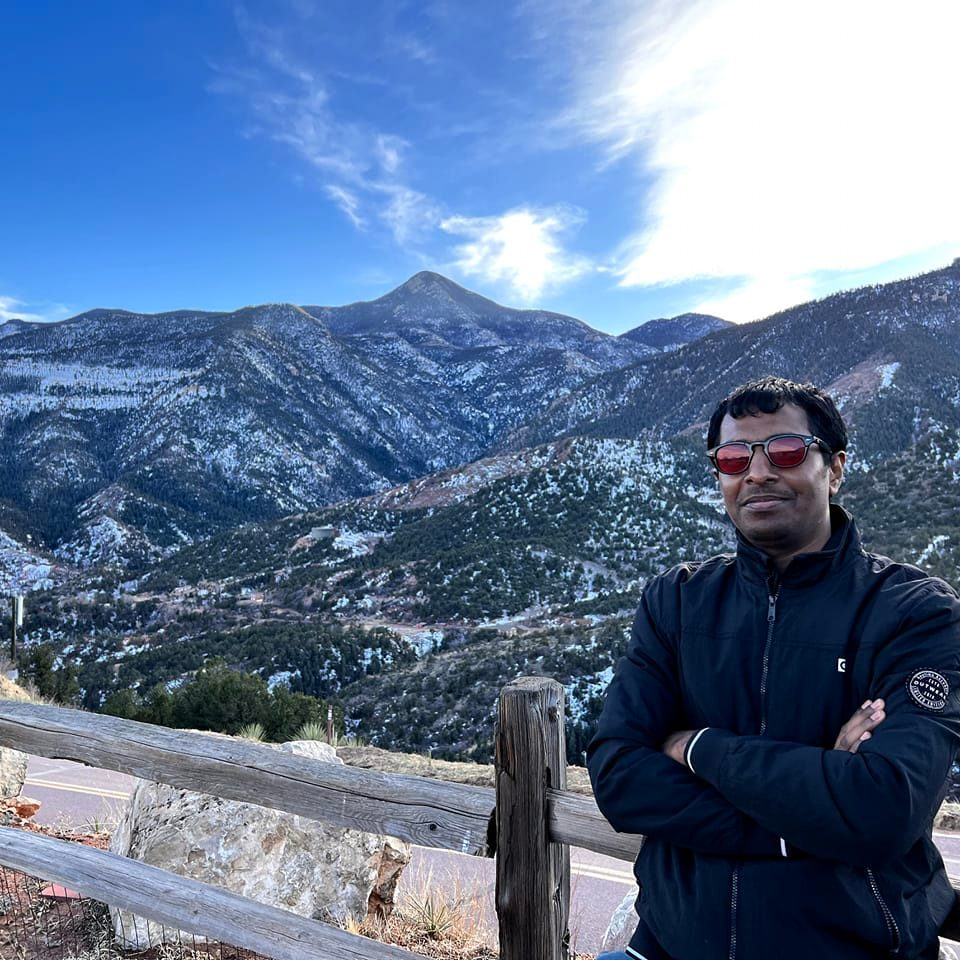
\includegraphics[width=.5\columnwidth]{picture-nazmus.jpg}
\caption{Picture of Nazmus.}
\label{fig:my-picture}
\end{figure}

\section{Introduction}

Hello. This is my immense pleasure to introduce myself here. My name is Nazmus Sakib, and I am from Bangladesh. I am a first-year Ph.D. student studying in the Cybersecurity program at the Computer Science Department at the University of Colorado Colorado Springs. I obtained a research-based Master of Computer Science degree from the University of Malaya, Malaysia in 2020. Prior to that, in 2012, I graduated with a B.Sc. (Engineering) in Computer Science and Engineering degree from the Shahjalal University of Science and Technology, Bangladesh. Currently, I am working as a Graduate Research Assistant (GRA) at the Networked System Security Lab at UCCS under Dr. Sang-Yoon Chang's supervision. I am interested in working in diverse computer science research fields including Blockchain, Bitcoin, Anomaly Detection, and Machine Learning.

\section{Related code}

I have been working on a research project titled ``Bitcoin Network Performance Analysis Using Annonymous Routing''. Here, we have logged Bitcoin Peer-to-Peer network and collect networking data.
Check the git repo here: https://github.com/peer-connectivity-estimator/bitcoin-network-logger

\section{Ask question here}

\subsection{Alharbi: How can user privacy concerns be addressed when using Bitcoin?}